\documentclass[12pt,letterpaper]{article}

% Idioma y codificación
\usepackage[utf8]{inputenc}
\usepackage[spanish,es-tabla]{babel}
\usepackage{lmodern}

% Márgenes y formato
\usepackage[left=3cm,right=2.5cm,top=3cm,bottom=3cm]{geometry}
\usepackage{fancyhdr}
\usepackage{float}
\pagestyle{fancy}
\fancyhf{}
\fancyhead[L]{Bitácora de Proyecto}
\fancyhead[R]{\thepage}

% Tablas y listas
\usepackage{longtable}
\usepackage{array}
\usepackage{multirow}
\usepackage{booktabs}
\usepackage{enumitem}

% Figuras y colores
\usepackage{graphicx}
\usepackage{xcolor}
\usepackage{caption}
\captionsetup[figure]{justification=centering}

% Hipervínculos
\usepackage[colorlinks=true, linkcolor=blue, urlcolor=blue, citecolor=black]{hyperref}

% Bibliografía
\usepackage[backend=bibtex,style=ieee,biblabel=dot]{biblatex}
\addbibresource{references.bib}

% Estilo de secciones
\usepackage{titlesec}
\titleformat*{\section}{\bfseries\large}
\titleformat*{\subsection}{\bfseries\normalsize}

%%%%%%%%%%%%%%%%%%%%%%%%%%%%%%%%%%%%%%%%%%%%
%                Documento                 %
%%%%%%%%%%%%%%%%%%%%%%%%%%%%%%%%%%%%%%%%%%%%
\begin{document}

% Portada
\begin{center}
    \textbf{\LARGE{Bitácora del Proyecto/Taller}} \\[6mm]
    \textbf{\large{Puerta con contraseña / Diseño de un decodificador}} \\[4mm]
    \textbf{\large{Fundamentos de Arquitectura de Computadores (CE 1107)}} \\[4mm]
    \textbf{\large{Instituto Tecnológico de Costa Rica}} \\[6mm]

    % Integrantes centrados
    \textbf{Integrantes:} \\[4mm]
    Emanuel Chavarría Hernández — 2022205841 \\[2mm]
    Fernando Fuchs Mora — 2020144908

    \textbf{\today}\\[8mm]
    \textbf{Repositorio:} \\[2mm]
    \url{https://github.com/Emanuel624/Bitacora_proyectofunda1_ECH_FFM}
\end{center}


%%%%%%%%%%%%%%%%%%%%%%%%%%%%%%%%%%%%%%%%%%%%
%              Entradas de bitácora        %
%%%%%%%%%%%%%%%%%%%%%%%%%%%%%%%%%%%%%%%%%%%%

\section{Sesión 1 -- 29 de agosto de 2025}
\subsection*{Actividades realizadas}
\begin{itemize}
    \item Se creó el repositorio para guardar y actualizar la presente bitácora.
    \item Como grupo se acordó leer los requerimientos del proyecto para llegar con dudas al profesor en la próxima clase o por medios virtuales.
\end{itemize}

\subsection*{Resultados obtenidos}
Se comenzó con el desarrollo del proyecto en una etapa básica.

\subsection*{Próximos pasos}
\begin{itemize}
    \item Comenzar con el proceso de simulación.
    \item Definir la tecnología que se va a utilizar.
    \item Definir el programa de simulación antes de construir el circuito.
\end{itemize}

\newpage

\section{Sesión 2 -- 30 de agosto de 2025}
\subsection*{Actividades realizadas}
\begin{itemize}
    \item Se comenzó con la investigación general de cómo desarrollar el proyecto y cuáles son los objetivos de realización.
    \item Se aclararon dudas iniciales del grupo sobre el proyecto con el profesor.
    \item Se compraron dos sensores de choque (\textit{shock}) de manera preliminar para comprobar si sirven para los objetivos del proyecto.
\end{itemize}

\begin{figure}[H]
    \centering
    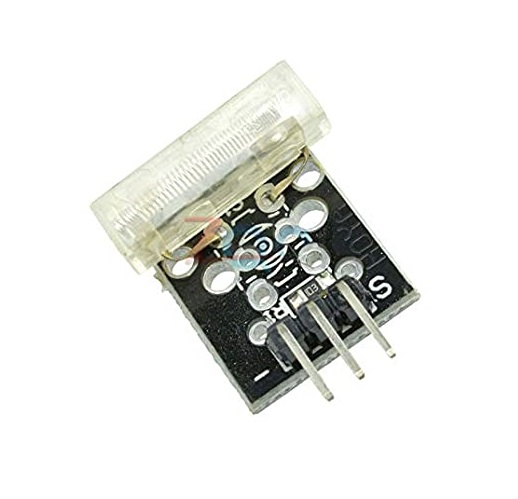
\includegraphics[width=0.3\textwidth]{images/sensor.jpg} % ruta del archivo
    \caption{Sensores de choque adquiridos para el proyecto.}
    \label{fig:sensores}
\end{figure}

\subsection*{Resultados obtenidos}
Se generó un plan de trabajo inicial.

\subsection*{Próximos pasos}
\begin{itemize}
    \item Se definió que el estudiante Emanuel Chavarría Hernández va a comenzar con el proceso inicial de realización de la simulación.
    \item Se puso en pausa el trabajo en el proyecto para atender otras responsabilidades académicas por parte de los integrantes.
\end{itemize}

\section{Sesión 3 -- 4 de septiembre de 2025}
\subsection*{Actividades realizadas}
\begin{itemize}
    \item Se definió el uso del programa Logisim-Evolution para la simulación.
    \item Surgieron nuevas dudas, esperando ser resueltas por parte del profesor.
    \item Se definió un circuito serializador, a la espera de ser aprobado por el profesor. Utilizando el circuito integrado 74LS164 de primera manera simulado, como se muestra en la siguiente figura, para comprobar el funcionamiento
\end{itemize}

\subsection*{Resultados obtenidos}
Se contó con el circuito serializador de manera preliminar, simulado.
\begin{figure}[H]
    \centering
    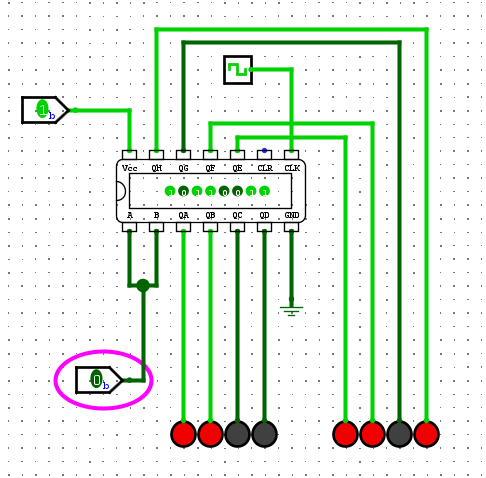
\includegraphics[width=0.3\textwidth]{images/serializador_sim.png} % ruta del archivo
    \caption{Circuito serializador simulado en Logisim-Evolution}
    \label{fig:serializador_sim}
\end{figure}

\subsection*{Próximos pasos}
\begin{itemize}
    \item Resolver las dudas con el profesor lo más pronto posible.
    \item Definir qué circuitos integrados comprar, tanto para serializador, compuerta y BCD.
    \item Trabajar simultáneamente tanto en el taller como en el proyecto.
\end{itemize}

\section{Sesión 4 -- 8 de septiembre de 2025}
\subsection*{Actividades realizadas}
\begin{itemize}
    \item Se resolvieron las dudas con el profesor.
    \item Se comenzó con la construcción del circuito combinatorio para reconocer el patrón por medio de simulación.
    \item Se definió el BCD a utilizar en el proyecto/taller.
    \item Se planteó el uso de 7 segmentos y como plantear la lógica.
\end{itemize}

\subsection*{Resultados obtenidos}
De manera especifica se va a mostrar el desarrollo teorico para el proceso del circuito combinatorio para recibir la contraseña de abrir y cerrar la puerta.
\section*{Definición de los Patrones}
El sistema debe reconocer dos patrones de entrada:

\begin{itemize}
  \item \textbf{Abrir}: El patrón de \textbf{Abrir} es \texttt{10110011}, donde:
    \begin{itemize}
      \item $Q_7 = 1$
      \item $Q_6 = 0$
      \item $Q_5 = 1$
      \item $Q_4 = 1$
      \item $Q_3 = 0$
      \item $Q_2 = 0$
      \item $Q_1 = 1$
      \item $Q_0 = 1$
    \end{itemize}
  \item \textbf{Cerrar}: El patrón de \textbf{Cerrar} es \texttt{11101000}, donde:
    \begin{itemize}
      \item $Q_7 = 1$
      \item $Q_6 = 1$
      \item $Q_5 = 1$
      \item $Q_4 = 0$
      \item $Q_3 = 1$
      \item $Q_2 = 0$
      \item $Q_1 = 0$
      \item $Q_0 = 0$
    \end{itemize}
\end{itemize}

\section*{Tabla de Verdad}

A continuación se presenta la tabla de verdad que muestra las combinaciones de las entradas \( Q_7, Q_6, \ldots, Q_0 \) y las salidas correspondientes **ABRIR** y **CERRAR**.

\[
\begin{array}{|c|c|c|c|c|c|c|c|c|c|}
\hline
Q_7 & Q_6 & Q_5 & Q_4 & Q_3 & Q_2 & Q_1 & Q_0 & \text{ABRIR} & \text{CERRAR} \\
\hline
1 & 0 & 1 & 1 & 0 & 0 & 1 & 1 & 1 & 0 \\
1 & 1 & 1 & 0 & 1 & 0 & 0 & 0 & 0 & 1 \\
\hline
\end{array}
\]

\section*{Desarrollo de la Lógica Combinatoria}

\subsection*{Ecuación para el patrón \textit{Abrir}}
El patrón de entrada para abrir la puerta es \texttt{10110011}. La ecuación lógica para detectar este patrón es la siguiente:

\[
\text{ABRIR} = Q_7 \cdot \neg Q_6 \cdot Q_5 \cdot Q_4 \cdot \neg Q_3 \cdot \neg Q_2 \cdot Q_1 \cdot Q_0
\]

\subsection*{Ecuación para el patrón \textit{Cerrar}}
El patrón de entrada para cerrar la puerta es \texttt{11101000}. La ecuación lógica para detectar este patrón es la siguiente:

\[
\text{CERRAR} = Q_7 \cdot Q_6 \cdot Q_5 \cdot \neg Q_4 \cdot Q_3 \cdot \neg Q_2 \cdot \neg Q_1 \cdot \neg Q_0
\]

\subsection*{Próximos pasos}
Gracias a las ecuaciones obtenidas por medio de suma de productos con las tablas de verdad, se llego al siguiente ciruicuito combinatorio para reconocer las contraseñas.
\begin{figure}[H]
    \centering
    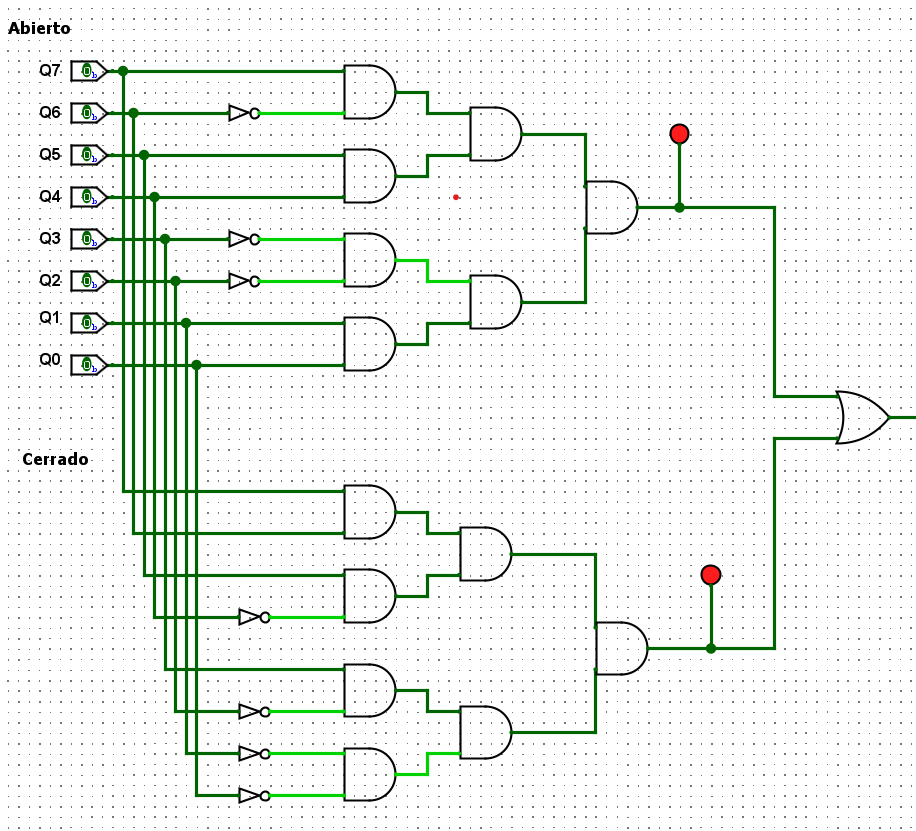
\includegraphics[width=0.3\textwidth]{images/sim_decodifcador.png} % ruta del archivo
    \caption{Circuito decodificador ABRIR y CERRAR la puerta simulado}
    \label{fig:sensores}
\end{figure}
Donde se resalta que las señales simplemente se unen con una compuerta AND para obtener una sola señal de salida. Y tiene un LED para mostrar cuando llega señal de 1 lógico o no.

\subsection*{Próximos pasos}
\begin{itemize}
    \item Confirmar el uso del 7 segmentos y como representar cada estado.
    \item Definir materiales por comprar para montar el circuito de manera física.
\end{itemize}

\section{Sesión 5 -- 9 de septiembre de 2025}
\subsection*{Actividades realizadas}
\begin{itemize}
    \item Se resolvieron problemas con la representación en el 7 segmentos, logrando usar $A$ para abrir y $C$ para cerrar.
    \item Se definió el uso de la tecnología TTL para el resto del proyecto.
    \item Se añadieron los archivos de simulación al repositorio dedicado al proyecto, para un mejor manejo de versiones.
\end{itemize}

\subsection*{Resultados obtenidos}
Se realizó la representación de la $A$ y $C$. Siguiendo la logica del BCD (74LS48) y del circuito como tal, se propuso el uso de una compuerta XOR, para lograr representar en cada caso cuando fuese necesario una $A$ y un $C$
\begin{figure}[H]
    \centering
    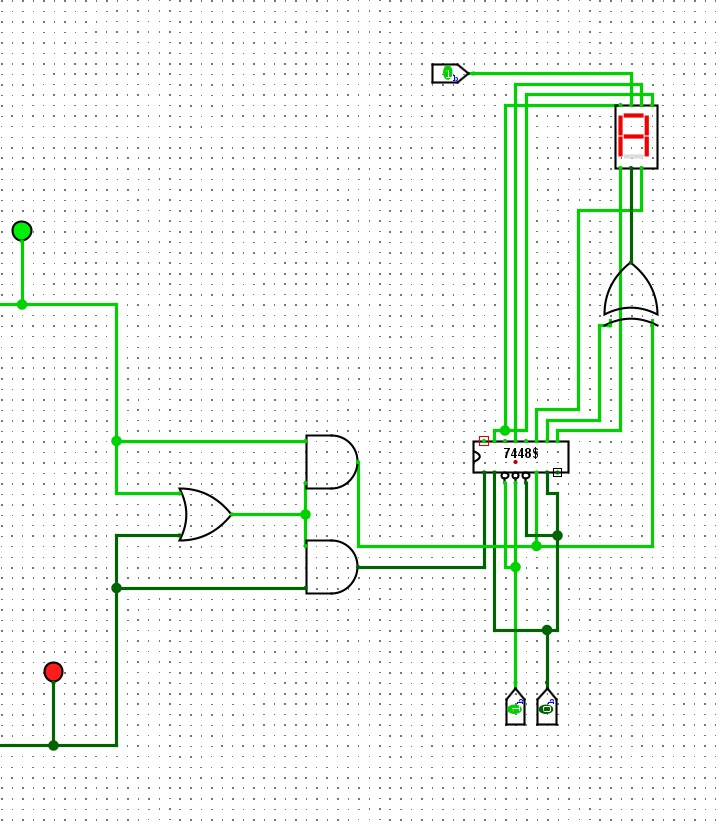
\includegraphics[width=0.3\textwidth]{images/bcd_mod.png} % ruta del archivo
    \caption{Circuito BCD simulado}
    \label{fig:sensores}
\end{figure}

\subsection*{Próximos pasos}
\begin{itemize}
    \item El estudiante Fernando Fuchs trabajará en montar el circuito en la herramienta Tinkercad para mayor facilidad a la hora de construirlo en físico.
    \item Se definió comprar los materiales entre el 10 y el 11 de septiembre.
    \item El estudiante Fernando Fuchs trabajará en las tareas restantes (investigar sobre el motor y accionador de puerta, etc.).
\end{itemize}


\section{Sesión 6 -- 9 de septiembre de 2025}
\subsection*{Actividades realizadas}
\begin{itemize}
    \item Se monta el circuito combinatorio para las contraseñas en la herramiente Tinkercad.
\end{itemize}

\subsection*{Resultados obtenidos}
\begin{figure}[H]
    \centering
    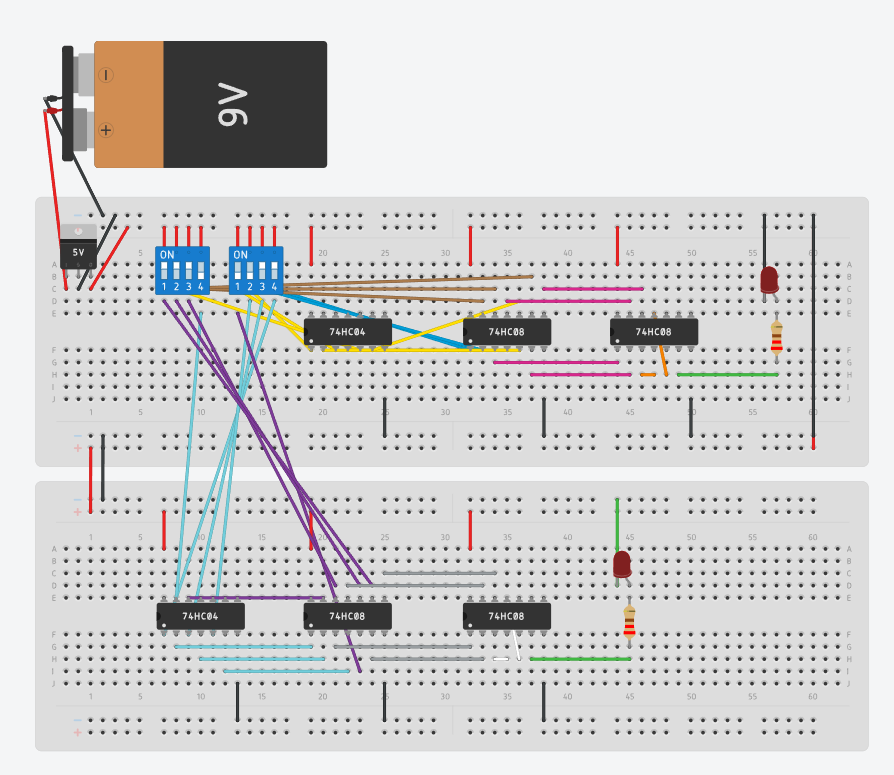
\includegraphics[width=0.3\textwidth]{images/tinkercad.png} % ruta del archivo
    \caption{Circuito en Tinkercad}
    \label{fig:tinkercad}
\end{figure}

\subsection*{Próximos pasos}
\begin{itemize}
    \item El estudiante Fernando Fuchs montará el circuito en físico.
\end{itemize}


\section{Sesión 7 -- 10-11 de septiembre de 2025}
\subsection*{Actividades realizadas}
\begin{itemize}
    \item Se monta el circuito combinatorio para las contraseñas en físico
\end{itemize}

\subsection*{Resultados obtenidos}
\begin{figure}[H]
    \centering
    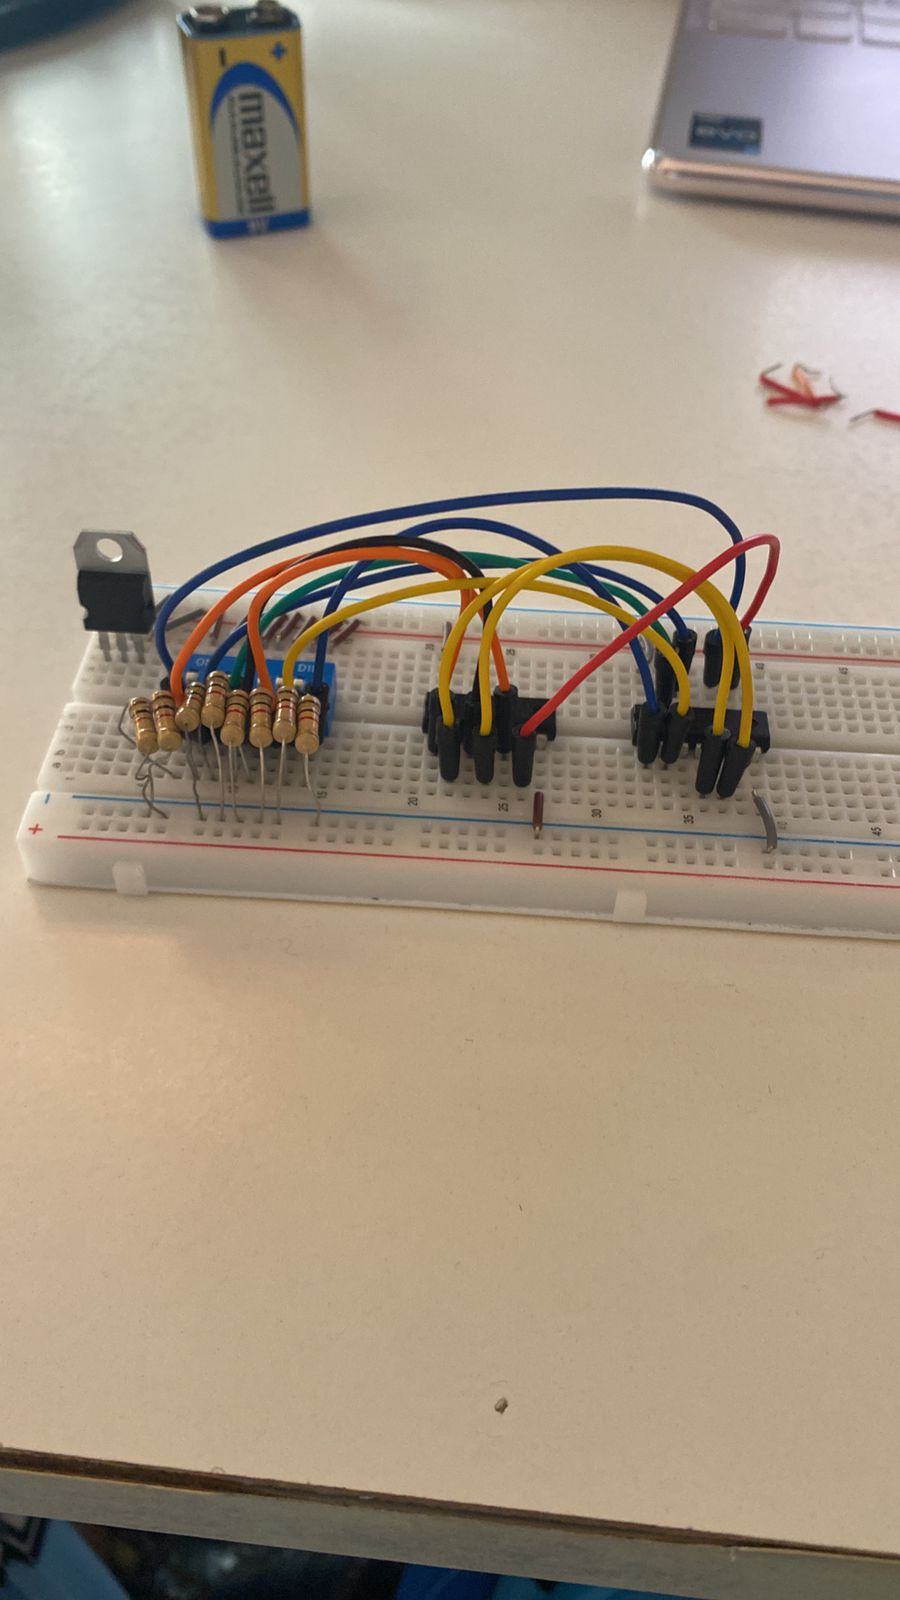
\includegraphics[width=0.2\textwidth]{images/fuchs1.jpg} % ruta del archivo
    \caption{Circuito en Protoboard}
    \label{fig:tinkercad}
\end{figure}
Se aclara, que se tuvieron problemas iniciales, debido a una mala conexión de resistencias de pulldown, así como mal uso del GND común, pero gracias a ayuda del profesor y de materiales consultados, se pudo realizar la correcta conexión de los circuitos combinatorios.

\subsection*{Próximos pasos}
\begin{itemize}
    \item El estudiante Emanuel Chavarría Hernandez montará el circuito del BCD.
\end{itemize}


\section{Sesión 8 -- 13-15 de septiembre de 2025}
\subsection*{Actividades realizadas}
\begin{itemize}
    \item Se monta el circuito combinatorio  + el circuito relacionado con el BCD y su representación con el 7 segmentos.
\end{itemize}

\subsection*{Resultados obtenidos}
\begin{figure}[H]
    \centering
    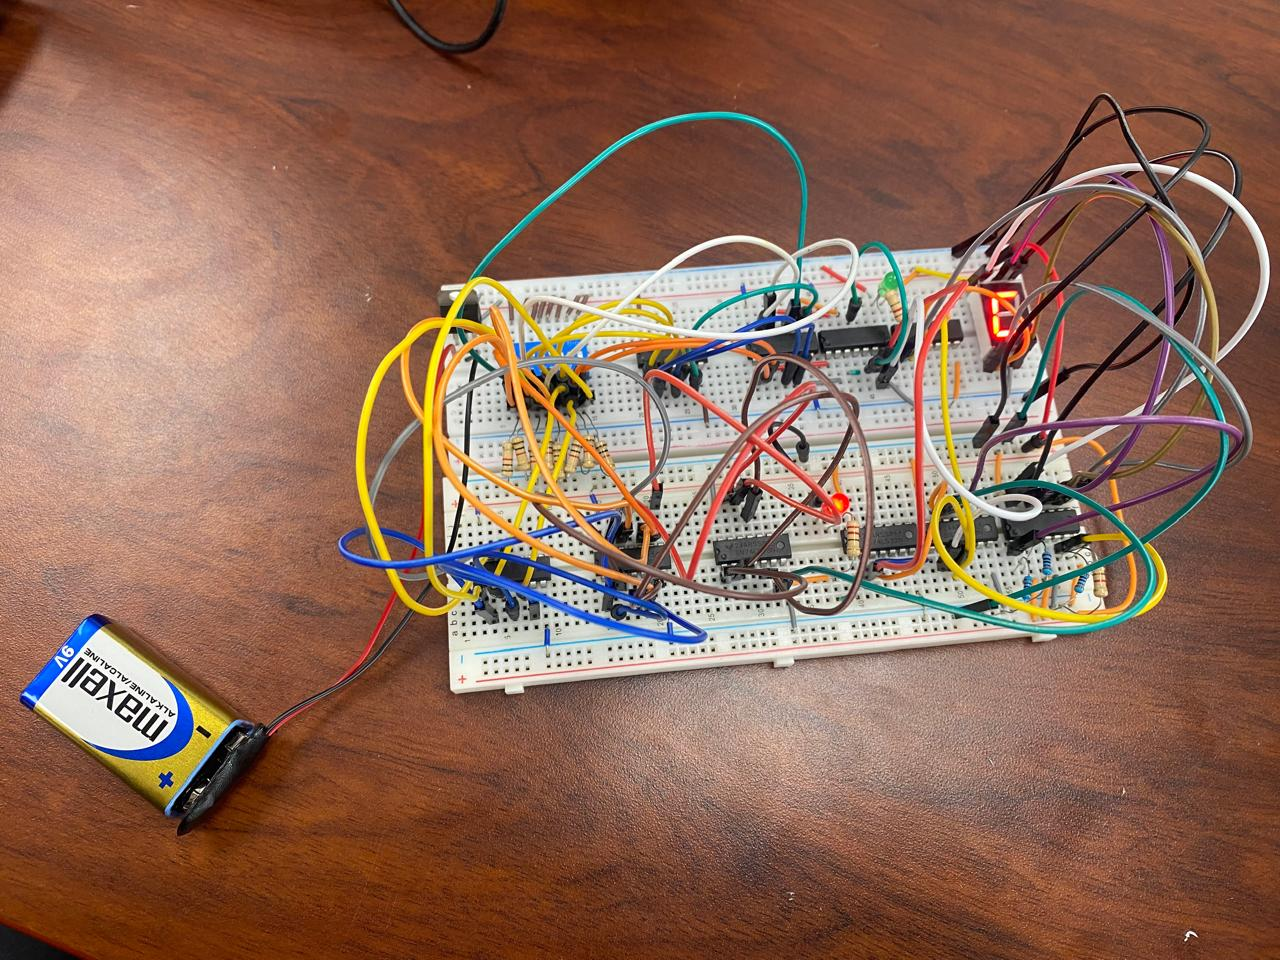
\includegraphics[width=0.3\textwidth]{images/todo_real.jpg} % ruta del archivo
    \caption{Circuito Completo}
    \label{fig:todo_taller}
\end{figure}
Se aclara, que con la conexión del BCD se tuvieron problemas, pero de nuevo, consultando materiales se resolvieron los problemas.

\subsection*{Próximos pasos}
\begin{itemize}
    \item Se termina la primera entrega del taller.
    \item Se sigue con la implementación total del proyecto a manos de Emanuel Chavarría Hernandez y Fernando Fuchs Mora. Falta por terminar, el motor, los sensores y el serializador todo en conjunto.
\end{itemize}
\end{document}
